\documentclass[aspectratio=169,12pt]{beamer}
\usepackage[utf8]{inputenc}
\usepackage{amsmath, amssymb}
\usepackage{booktabs}
\usepackage{colortbl}
\usepackage{hyperref}
\usepackage{makecell}
\usepackage{ragged2e}
\usepackage{tikz}
\usetikzlibrary{arrows.meta, positioning, shapes.geometric, calc, tikzmark, shapes.misc, fit, decorations.pathreplacing, matrix}
\usepackage{tcolorbox}
\usepackage{array}
\usepackage{listings}
\usepackage{pgfkeys}
\usepackage{adjustbox}
\usepackage[normalem]{ulem} 
\usetheme{Madrid}
\usecolortheme{default}

% Custom colors
\definecolor{mygreen}{RGB}{0,150,0}
\definecolor{myblue}{RGB}{0,100,200}
\definecolor{myred}{RGB}{200,0,0}
\definecolor{mygray}{RGB}{100,100,100}

\title{Computer Structure}
\subtitle{X86 Virtual Memory and TLB}
\author{}
\date{}

\begin{document}

\begin{frame}
\titlepage
\end{frame}

% Slide 2: X86 Paging Introduction
\begin{frame}{X86 Paging}
\begin{itemize}
    \item For 32-bit addressing with 4KB page size, a full page table would require 4MB
    \item Most processes use only a small amount of memory
    \item The overhead of 4MB per process is expensive and unnecessary
    \item In X86, there are multiple levels of translation tables organized in a tree structure
    \item We allocate translation tables dynamically, only when actually needed
\end{itemize}
\end{frame}

% Slide 3: 32-bit Mode Page Mapping
\begin{frame}{32-bit Mode: 4KB / 4MB Page Mapping}
\begin{itemize}
    \item 2-level hierarchical mapping: Page Directories and Page Tables
    \item 4KB aligned pages
    \item PDE (Page Directory Entry) contains:
    \begin{itemize}
        \item Present bit (0 = page fault)
        \item Page size (4KB or 4MB)
        \item CR4.PSE=1 $\Rightarrow$ both 4MB \& 4KB pages supported
        \item Separate TLBs for different page sizes
    \end{itemize}
\end{itemize}

\vspace{1em}
Linear Address Space breakdown:
\begin{itemize}
    \item 4KB Page: DIR[31:22] | TABLE[21:12] | OFFSET[11:0]
    \item 4MB Page: DIR[31:22] | OFFSET[21:0]
\end{itemize}
\end{frame}

% Slide 4: PDE and PTE Format
\begin{frame}{32-bit Mode: PDE and PTE Format}
\centering
\textbf{Page Directory Entry (4KB page table)}\\[0.5em]
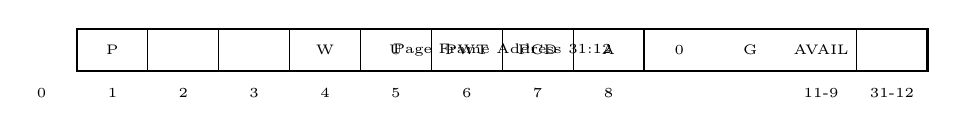
\begin{tikzpicture}[scale=0.9]
    % PDE structure
    \draw[thick] (0,0) rectangle (12,0.6);
    \foreach \x/\txt in {0/0,1/1,2/2,3/3,4/4,5/5,6/6,7/7,8/8,11/{11-9},12/{31-12}} {
        \draw (\x,0) -- (\x,0.6);
        \node[below] at (\x-0.5,-0.1) {\tiny \txt};
    }
    \node at (6,0.3) {\tiny Page Frame Address 31:12};
    \node at (10.5,0.3) {\tiny AVAIL};
    \node at (9.5,0.3) {\tiny G};
    \node at (8.5,0.3) {\tiny 0};
    \node at (7.5,0.3) {\tiny A};
    \node at (6.5,0.3) {\tiny PCD};
    \node at (5.5,0.3) {\tiny PWT};
    \node at (4.5,0.3) {\tiny U};
    \node at (3.5,0.3) {\tiny W};
    \node at (0.5,0.3) {\tiny P};
\end{tikzpicture}

\vspace{1em}
\textbf{Page Table Entry}\\[0.5em]
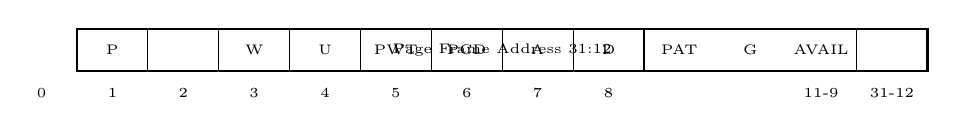
\begin{tikzpicture}[scale=0.9]
    % PTE structure
    \draw[thick] (0,0) rectangle (12,0.6);
    \foreach \x/\txt in {0/0,1/1,2/2,3/3,4/4,5/5,6/6,7/7,8/8,11/{11-9},12/{31-12}} {
        \draw (\x,0) -- (\x,0.6);
        \node[below] at (\x-0.5,-0.1) {\tiny \txt};
    }
    \node at (6,0.3) {\tiny Page Frame Address 31:12};
    \node at (10.5,0.3) {\tiny AVAIL};
    \node at (9.5,0.3) {\tiny G};
    \node at (8.5,0.3) {\tiny PAT};
    \node at (7.5,0.3) {\tiny D};
    \node at (6.5,0.3) {\tiny A};
    \node at (5.5,0.3) {\tiny PCD};
    \node at (4.5,0.3) {\tiny PWT};
    \node at (3.5,0.3) {\tiny U};
    \node at (2.5,0.3) {\tiny W};
    \node at (0.5,0.3) {\tiny P};
\end{tikzpicture}

\vspace{1em}
\small
Key: P=Present, W=Writable, U=User/Supervisor, PWT=Write-Through,\\
PCD=Cache Disable, A=Accessed, D=Dirty, G=Global, PAT=Page Attribute Table
\end{frame}

% Slide 5: 64-bit Mode Page Mapping
\begin{frame}{4KB Page Mapping in 64-bit Mode}
\begin{itemize}
    \item Introduced in 2003 with AMD Opteron
    \item 4-level hierarchy: PML4, PDP, DIR, TABLE
    \item 512 entries per table (9 bits addressing)
    \item 48 bits of virtual address space (256 TB)
    \item 40 bits of physical address space (1 TB)
\end{itemize}

\vspace{1em}
Linear Address breakdown (4KB page):\\
\texttt{[63:48] Sign Ext | [47:39] PML4 | [38:30] PDP | [29:21] DIR | [20:12] TABLE | [11:0] OFFSET}
\end{frame}

% Slide 6: Large Pages in 64-bit Mode
\begin{frame}{Large Pages in 64-bit Mode}
\textbf{2MB Page Mapping:}
\begin{itemize}
    \item Linear Address: Sign Ext | PML4[47:39] | PDP[38:30] | DIR[29:21] | OFFSET[20:0]
    \item Page size: $2^{21}$ = 2MB
\end{itemize}

\vspace{1em}
\textbf{1GB Page Mapping:}
\begin{itemize}
    \item Linear Address: Sign Ext | PML4[47:39] | PDP[38:30] | OFFSET[29:0]
    \item Page size: $2^{30}$ = 1GB
\end{itemize}
\end{frame}

% Slide 7: Question 1 Setup
\begin{frame}{Question 1}
Core similar to X86 in 64-bit mode:
\begin{itemize}
    \item Support Small Pages (PTE) and Large Pages (DIR)
    \item Page table size = small page size
    \item Entry size in all hierarchies = 16 bytes
\end{itemize}

\vspace{0.5em}
Address format:\\
\texttt{[63:N4+1] Sign Ext | [N4:N3+1] PML4 | [N3:N2+1] PDP | [N2:N1+1] DIR | [N1:12] TABLE | [11:0] OFFSET}

\vspace{0.5em}
\textbf{Questions:}
\begin{enumerate}
    \item What is the size of a small page?
    \item How many entries are in each Page Table?
    \item What are the values of N1, N2, N3, and N4?
    \item What is the size of a large page?
\end{enumerate}
\end{frame}

% Slide 8: Question 1 Solution
\begin{frame}{Question 1 - Solution}
\textbf{1. Small page size:}
\begin{itemize}
    \item 12 bits in offset field $\Rightarrow 2^{12}$ = 4KB
\end{itemize}

\textbf{2. Entries per Page Table:}
\begin{itemize}
    \item Page Table size = Page Size = 4KB
    \item PTE = 16B
    \item Entries = 4KB / 16B = $2^{12} / 2^4 = 2^8$ = 256 entries
\end{itemize}

\textbf{3. Values of N1, N2, N3, N4:}
\begin{itemize}
    \item 256 entries $\Rightarrow$ 8 bits to address them
    \item TABLE [19:12] $\Rightarrow$ N1 = 19
    \item DIR [27:20] $\Rightarrow$ N2 = 27
    \item PDP [35:28] $\Rightarrow$ N3 = 35
    \item PML4 [43:36] $\Rightarrow$ N4 = 43
\end{itemize}

\textbf{4. Large page size:}
\begin{itemize}
    \item Large pages pointed by DIR, offset is [19:0]
    \item Size = $2^{20}$ = 1MB
\end{itemize}
\end{frame}

% Slide 9: TLB Introduction
\begin{frame}{Translation Lookaside Buffer (TLB)}
\begin{itemize}
    \item Page table resides in memory
    \item Each translation requires extra memory access
    \item TLB caches recently used PTEs to speed up translation
    \item Typically 128-256 entries, 4-8 way associative
\end{itemize}

\vspace{1em}
\textbf{TLB Operation:}
\begin{enumerate}
    \item Virtual address presented for translation
    \item Check TLB for matching VPN
    \item \textbf{TLB Hit:} Use cached translation
    \item \textbf{TLB Miss:} Page Miss Handler (PMH) fetches PTE from memory
\end{enumerate}
\end{frame}

% Slide 10: Virtual Memory and Cache
\begin{frame}{Virtual Memory and Cache}
\textbf{Access Flow:}
\begin{enumerate}
    \item TLB access is serial with cache access
    \item Page table entries are cached in L1 D\$, L2\$, and L3\$ as data
\end{enumerate}

\vspace{1em}
\textbf{On memory access:}
\begin{itemize}
    \item First check TLB/STLB
    \item If TLB miss, perform page walk
    \item Access cache hierarchy with physical address
    \item If cache miss, access main memory
\end{itemize}

\vspace{1em}
\textbf{TLB Types:}
\begin{itemize}
    \item Separate TLBs for data (dTLB) and instructions (iTLB)
    \item Separate TLBs for 4KB and large page sizes
    \item STLB (Secondary TLB) as second level
\end{itemize}
\end{frame}

% Slide 11: Page Walk and PMH
\begin{frame}{Page Walk Process}
\textbf{PMH (Page Miss Handler) Operation:}
\begin{itemize}
    \item PMH performs page walk on TLB miss
    \item Walks the page table hierarchy from root (PML4)
    \item PMH contains caches for higher translation levels:
    \begin{itemize}
        \item PML4 cache
        \item PDP cache
        \item DIR cache
    \end{itemize}
\end{itemize}

\vspace{1em}
\textbf{PMH Cache Access:}
\begin{center}
\begin{tabular}{|l|c|c|}
\hline
\textbf{Cache} & \textbf{Accessed with} & \textbf{Returns} \\
\hline
DIR cache & [47:21] & PDE \\
PDP cache & [47:30] & PDP entry \\
PML4 cache & [47:39] & PML4 entry \\
\hline
\end{tabular}
\end{center}

\vspace{0.5em}
Note: No Table cache needed as TLB stores complete translations
\end{frame}

% Slide 12: Question 2 Setup
\begin{frame}{Question 2}
\textbf{System Configuration:}
\begin{itemize}
    \item Processor similar to X86 - 64 bits
    \item 4KB pages
    \item TLB present (Hit: immediate translation, Miss: Page Walk required)
    \item PMH contains cache for each translation table level
    \item All caches and TLB empty on reset
\end{itemize}

\vspace{1em}
\textbf{Memory Access Sequence:}
\begin{center}
\begin{tabular}{|l|c|l|}
\hline
\textbf{Address} & \textbf{Memory Accesses} & \textbf{Explanation} \\
\hline
0x0000022334455666 & ? & \\
0x0000022334455777 & ? & \\
0x0000022884455777 & ? & \\
\hline
\end{tabular}
\end{center}
\end{frame}

% Slide 13: Question 2 Solution
\begin{frame}{Question 2 - Solution}
\begin{center}
\begin{tabular}{|l|c|p{6cm}|}
\hline
\textbf{Address} & \textbf{Accesses} & \textbf{Explanation} \\
\hline
0x0000022334455666 & 4 & Need to access memory for each of the 4 translation tables \\
\hline
0x0000022334455777 & 0 & Same page as above $\Rightarrow$ TLB hit $\Rightarrow$ No memory access \\
\hline
0x0000022884455777 & 3 & Hit in PML4 cache, then miss in PDP. Need to access memory 3 times: PDP, DIR, PTE \\
\hline
\end{tabular}
\end{center}
\end{frame}

% Slide 14: Cache Design Question
\begin{frame}{Question 2: Cache Design}
\textbf{System Configuration:}
\begin{itemize}
    \item Virtual address: 48 bits
    \item Physical address: 41 bits
    \item L1 data cache: 32KB, 2-way set associative, 64B line size
\end{itemize}

\vspace{1em}
\textbf{Question:} How can we access this cache before getting the physical address?

\vspace{1em}
\textbf{Analysis:}
\begin{itemize}
    \item 64B lines $\Rightarrow$ 6 offset bits [5:0]
    \item 32KB / (2 ways × 64B) = 256 sets $\Rightarrow$ 8 set bits [13:6]
    \item 12 bits [11:0] are not translated (page offset)
    \item We lack 2 bits [13:12] for complete set address
    \item Solution: Use untranslated bits [13:12] for set lookup
    \item Must compare entire PFN with tag due to aliasing possibility
\end{itemize}
\end{frame}

% Slide 15: Virtual Aliasing Problem
\begin{frame}{Virtual Aliasing Problem}
\textbf{Problem:} Two virtual pages mapping to same physical page

\vspace{1em}
Example:
\begin{itemize}
    \item VPN xxxx01 $\rightarrow$ PFN zzzz
    \item VPN yyyy00 $\rightarrow$ PFN zzzz
    \item Bits [13:12] differ (01 vs 00)
\end{itemize}

\vspace{1em}
\textbf{Consequence:}
\begin{itemize}
    \item Same data may exist in two different cache sets
    \item Violates cache coherency
\end{itemize}

\vspace{1em}
\textbf{Solution:}
\begin{itemize}
    \item Check 4 possible sets when allocating new entry
    \item If same tag appears, evict the alias
    \item On snoop: must check 4 sets × 2 ways = 8 locations
\end{itemize}
\end{frame}

% Slide 16: Question 3 Setup
\begin{frame}{Question 3}
\textbf{System Configuration:}
\begin{itemize}
    \item Core similar to X86 in 64-bit mode
    \item Entry size in all page tables: 8 bytes
    \item PMH caches at all levels:
    \begin{itemize}
        \item 4 entries, direct mapped
        \item Hit time: 2 cycles
        \item Miss detected after 1 cycle
    \end{itemize}
    \item Main memory access: 100 cycles (not including miss detection)
    \item All PMH levels accessed in parallel
\end{itemize}

\vspace{1em}
Address format:\\
\texttt{[63:56] Sign | [55:36] PML4 | [35:24] PDP | [23:12] DIR | [11:0] TABLE/OFFSET}

\vspace{0.5em}
\textbf{Questions:}
\begin{enumerate}
    \item What is the large page size?
    \item How many entries in each table?
\end{enumerate}
\end{frame}

% Slide 17: Question 3 Solution Part 1
\begin{frame}{Question 3 - Solution Part 1}
\textbf{1. Large page size:}
\begin{itemize}
    \item Large pages pointed by DIR
    \item Offset bits: [23:0]
    \item Size = $2^{24}$ = 16MB
\end{itemize}

\vspace{1em}
\textbf{2. Entries per table:}
\begin{itemize}
    \item TABLE: $2^{12}$ bits offset $\Rightarrow 2^{12}$ entries
    \item DIR: $2^{12}$ bits $\Rightarrow 2^{12}$ entries  
    \item PDP: $2^{12}$ bits $\Rightarrow 2^{12}$ entries
    \item PML4: $2^{8}$ bits $\Rightarrow 2^{8}$ = 256 entries
\end{itemize}
\end{frame}

% Slide 18: Question 3 Memory Access Analysis
\begin{frame}{Question 3 - Memory Access Analysis}
\footnotesize
\begin{center}
\begin{tabular}{|l|c|p{7cm}|}
\hline
\textbf{Virtual Address} & \textbf{Cycles} & \textbf{Comment} \\
\hline
0xFF81234567​89ABCD & 401 & Miss at each level: 1 + 4×100 = 401 cycles \\
\hline
0xFF81234067​89ABCD & 202 & (PML4, PDP, DIR, TLB) = (H,H,M,M)\\
& & 1 cycle + PDP read 1 cycle\\
& & DIR miss: 100 cycles, PTE miss: 100 cycles \\
\hline
0xFF80234067​89ABCD & 401 & PMH cache miss in all levels: 1 + 4×100 = 401 \\
\hline
0xFF81234067​09ABCD & 302 & (PML4, PDP, DIR, TLB) = (H,M,M,M)\\
& & Entry 234 replaced by access 3 (same set)\\
& & 2 + 3×100 = 302 cycles \\
\hline
0xFF81234067​09A0CD & 2 & Hit in TLB - 2 cycles \\
\hline
\end{tabular}
\end{center}
\end{frame}

% Final slide
\begin{frame}
\centering
\Huge{Questions?}
\end{frame}

\end{document}